\documentclass[a4paper,twocolumn,11pt,unpublished]{quantumarticle}
\pdfoutput=1
\usepackage[utf8]{inputenc}
\usepackage[english]{babel}
\usepackage[T1]{fontenc}
\usepackage{amsmath,amssymb,amsthm,mathtools}
\usepackage{booktabs}
\usepackage{graphicx}
\usepackage{hyperref}
\usepackage{xcolor}

\newtheorem{theorem}{Theorem}
\newtheorem{proposition}[theorem]{Proposition}
\newtheorem{lemma}[theorem]{Lemma}
\newcommand{\DC}{\operatorname{DC}}
\newcommand{\Tr}{\operatorname{Tr}}

\begin{document}

\title{Recursive Binary Words as Dimension-Bounded Temporal Memory Witnesses}

\author{Youfu Wang}
\email{youfuwang888@gmail.com}
\orcid{0009-0005-5998-6024}
\affiliation{Independent Researcher, Anyang, China}

\maketitle

\begin{abstract}
How much internal memory is required for an autonomous device to emit a
specified temporal word when the same binary instrument is applied at every
step?  We answer this question for the dyadic finite Thue--Morse words
$T_n=\mu^n(0)$, with $\mu(0)=01$ and $\mu(1)=10$.  If the stopping length is
external and no clock, index, or round label enters the device, their exact
deterministic classical complexity is
$\DC(T_n)=3\,2^{n-2}=3|T_n|/4$ for every $n\geq2$.  At lengths eight and
sixteen we give machine-auditable global certificates for stationary
two-state classical generators and explicit stationary qubit instruments.
For $T_3=01101001$ the certified classical and quantum thresholds are
$P_{\mathrm C}<0.03<P_{\mathrm Q}$ with $P_{\mathrm Q}>0.0414$; for
$T_4=0110100110010110$ they are
$P_{\mathrm C}<0.0005<P_{\mathrm Q}$ with $P_{\mathrm Q}>0.00069$.
These establish equal-dimension temporal separations at two recursive
scales.  Under a registered reset-noise model for the length-eight test,
the separation persists up to a per-round noise rate of
$8.5449\ldots\%$; exact binomial calculations give concrete finite-sample
requirements.  The result is a dimension-bounded temporal-memory witness,
not a device-independent statement and not evidence for hidden quantum
states.
\end{abstract}

\section{Introduction}

Temporal correlations turn internal dimension into an operational memory
resource.  In the simplest stationary scenario, one finite-dimensional
system is subjected repeatedly to the same binary-output instrument
\cite{VieiraBudroni2022}.  A device with insufficient memory cannot generate
every requested word deterministically, and classical and quantum models of
the same dimension can assign different probabilities to the same temporal
event \cite{Brierley2015,Budroni2019}.  This provides a particularly lean
setting for dimension-bounded tests: there are no measurement choices and no
time-dependent controls inside the abstract model.

The recursive Thue--Morse words are a natural stress test for autonomous
memory.  Although the infinite sequence is $2$-automatic
\cite{AlloucheShallit2003}, the standard automaton reads the binary digits of
the time index.  Here the device receives no index or clock.  It must encode
progress through a finite target word in its internal state while the same
instrument is repeated (Fig.~\ref{fig:protocol}).  Thus two-automaticity does
not imply two-state autonomous generation.

\begin{figure*}[t]
  \centering
  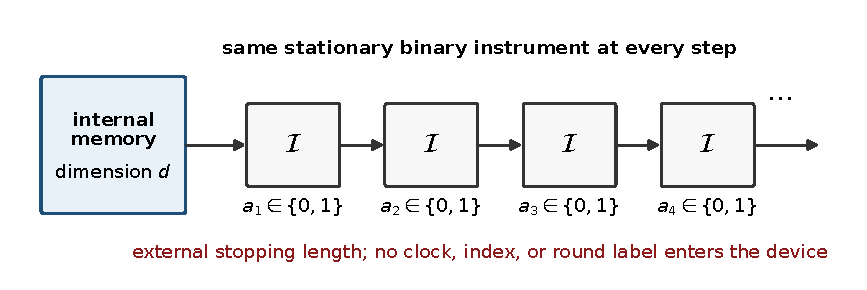
\includegraphics[width=0.98\textwidth]{figures/fig1_protocol.pdf}
  \caption{Operational task.  A memory of fixed dimension $d$ is subjected
  to the same stationary binary instrument $\mathcal I$ at every step.
  The experimenter stops after a prescribed external length, but no clock,
  index, position, or round label enters the device.}
  \label{fig:protocol}
\end{figure*}

\paragraph{Contributions and assumptions.}
Our contributions are fourfold.
\begin{enumerate}
  \item We prove an exact family theorem,
  $\DC(T_n)=3|T_n|/4$, for all dyadic finite Thue--Morse words.
  \item For $T_3$ and $T_4$, we certify global upper bounds on every
  stationary two-state classical generator.
  \item We provide explicit stationary qubit instruments above both bounds.
  The quantum probabilities are verified by outward interval arithmetic.
  \item We give a frozen noise model and exact-binomial power calculations
  for an implementation-oriented test.
\end{enumerate}
The separation assumes a stationary two-dimensional memory, a binary
instrument, and the absence of a hidden clock.  These are trusted-model
assumptions.  The result is neither device independent nor a claim about a
microscopic ontology.

The closest operational study is Ref.~\cite{VieiraBudroni2022}, which
introduced the deterministic complexity used here and numerically surveyed
classical words through length ten and quantum words through length seven.
Our contribution is word-specific and certificate-based: an exact recursive
family theorem, two certified recursive scales, and reproducible global
classical bounds.  Recent comparisons of one-bit and one-qubit finite-state
generators use different temporal scores and delayed measurement settings
\cite{Deb2026}.  Other temporal dimension witnesses
\cite{Brierley2015,Budroni2019,Ringbauer2017,Sohbi2021,Vieira2024},
hidden-memory tests \cite{Taranto2023}, and quantum stochastic simulators
\cite{Garner2017,Elliott2020} address related memory questions under
different operational tasks.

\section{Stationary temporal generators}
\label{sec:model}

Let $w=a_1\cdots a_L\in\{0,1\}^L$.  A classical generator of dimension $d$
is specified by nonnegative $d\times d$ matrices $T_0,T_1$ satisfying
\begin{equation}
  (T_0+T_1)\boldsymbol{1}=\boldsymbol{1}
  \label{eq:classicalnormalization}
\end{equation}
and an initial row distribution $\boldsymbol{\pi}$.  Its word probability is
\begin{equation}
  P_{\mathrm C}(w)=
  \boldsymbol{\pi}T_{a_1}\cdots T_{a_L}\boldsymbol{1}.
  \label{eq:classicalprob}
\end{equation}
The matrices jointly encode the emitted symbol and the memory transition.

A quantum generator of dimension $d$ is a density operator $\rho$ and a
binary instrument $\{\mathcal I_0,\mathcal I_1\}$, where each
$\mathcal I_a$ is completely positive and trace nonincreasing and
$\mathcal I_0+\mathcal I_1$ is trace preserving.  Its word probability is
\begin{equation}
  P_{\mathrm Q}(w)=
  \Tr\!\left[
  \mathcal I_{a_L}\circ\cdots\circ\mathcal I_{a_1}(\rho)
  \right].
  \label{eq:quantumprob}
\end{equation}
Both models are stationary: the same pair of maps is used at every step.
The stopping length $L$ is imposed externally.

A deterministic classical generator has one outgoing symbol-transition
from every reachable state.  Along a finite run its state path is a tail
followed by a cycle.  The deterministic complexity $\DC(w)$ is the minimum
number of states in such a generator that emits $w$ before the external stop
\cite{VieiraBudroni2022}.

\section{Exact deterministic complexity}
\label{sec:deterministic}

Define $\mu(0)=01$, $\mu(1)=10$, and
\begin{equation}
  T_n=\mu^n(0),\qquad N=|T_n|=2^n.
\end{equation}

\begin{theorem}[Finite Thue--Morse complexity]
\label{thm:dc}
For every $n\geq2$,
\begin{equation}
  \boxed{\DC(T_n)=3\,2^{n-2}=\frac{3N}{4}.}
  \label{eq:dc}
\end{equation}
The same formula holds for the bitwise complement $\overline{T_n}$.
\end{theorem}

The proof uses the longest repeated factor at a fixed displacement.  For a
finite word $w=w_0\ldots w_{N-1}$ define
\begin{equation}
\begin{split}
M(w)=\max\{\,\ell:\;&q\geq1,\ s\geq0,\ s+q+\ell\leq N,\\
&w_{s+j}=w_{s+q+j}\ \text{for }0\leq j<\ell\,\}.
\end{split}
\label{eq:selfmatch}
\end{equation}
For an odd displacement, no four consecutive symbols of the infinite
Thue--Morse word can agree: even-start and odd-start length-four factors
belong to disjoint finite sets.  For an even displacement $2r$, the
identities $t_{2i}=t_i$ and $t_{2i+1}=1-t_i$ duplicate every equality
indicator at displacement $r$.  Iterating this desubstitution and checking
the terminal words $T_1,T_2,T_3$ gives $M(T_n)\leq N/4$.
Conversely,
\begin{equation}
  T_n=A\,\overline A\,\overline A\,A,\qquad A=T_{n-2},
  \label{eq:fourblocks}
\end{equation}
so the prefix and suffix agree for $N/4$ symbols and
$M(T_n)=N/4$.

If a tail-cycle generator has $d$ states, then the final $N-d$ outputs repeat
an earlier block at the cycle displacement.  Hence
$N-d\leq M(T_n)=N/4$, so $d\geq3N/4$.  A cycle containing the first $3N/4$
symbols reproduces the final block $A$ in Eq.~\eqref{eq:fourblocks}, proving
attainability.  Appendix~\ref{app:proof} gives the finite-boundary details.
Figure~\ref{fig:dc} shows the resulting linear memory law.

\begin{figure}[t]
  \centering
  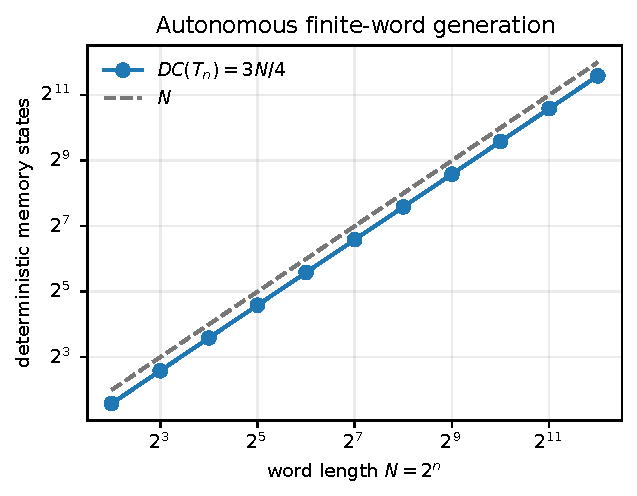
\includegraphics[width=\columnwidth]{figures/fig2_dc_scaling.pdf}
  \caption{Exact deterministic memory of $T_n$.  The standard
  two-state automatic description is not available here because it requires
  the binary digits of the time index as input.}
  \label{fig:dc}
\end{figure}

\section{Certified dimension-two separation}
\label{sec:separation}

We first fix the length-eight target
\begin{equation}
  w=T_3=01101001.
\end{equation}
Theorem~\ref{thm:dc} gives $\DC(w)=6$, so both dimension-two models operate
strictly below the deterministic threshold.

\subsection{Exact-rational classical upper bound}

For $d=2$, the initial distribution can be chosen pure because
Eq.~\eqref{eq:classicalprob} is linear in $\boldsymbol{\pi}$.  Relabelling the
two internal states then fixes $\boldsymbol{\pi}=(1,0)$ without loss of
generality.  The eight nonnegative entries of $T_0,T_1$, subject to the two
normalization equations in Eq.~\eqref{eq:classicalnormalization}, leave six
independent variables on a product of two simplices.

We cover this domain with rational boxes.  For every box, each independent
matrix entry is replaced by its rational upper endpoint, while the dependent
entry in each stochastic row is bounded by one minus the sum of the rational
lower endpoints.  Positivity of all matrices makes the resulting forward
propagation an upper bound on Eq.~\eqref{eq:classicalprob}.  Bisecting the
widest coordinate produces a nested cover.  After $130000$ bisections, the
largest exact bound over all $130001$ queued boxes is
\begin{equation}
  \frac{16282708641}{549755813888}
  =0.029618074479\ldots < \frac{3}{100}.
  \label{eq:exactcertificate}
\end{equation}
Because the queued boxes still cover the full feasible domain,
Eq.~\eqref{eq:exactcertificate} is a global certificate rather than a
variational estimate.  Appendix~\ref{app:certificate} states the algorithm
and its coverage invariant.

\subsection{Explicit qubit instrument}

Let $\rho=|\psi\rangle\langle\psi|$ with
\begin{equation}
|\psi\rangle=
\begin{pmatrix}\cos\theta\\ \sin\theta\end{pmatrix},
\qquad \theta=-0.2880903478104165,
\end{equation}
and define
\begin{equation}
K_0=
\begin{pmatrix}
-0.261100885994&-0.263277264622\\
 0.894987283427&-0.279312440034
\end{pmatrix},
\end{equation}
\begin{equation}
\begin{aligned}
K_1&=R(\phi)\sqrt{I-K_0^\top K_0},\\
\phi&=2.1351675998196673,
\end{aligned}
\end{equation}
where $R(\phi)$ is the real two-dimensional rotation.  The residual
$I-K_0^\top K_0$ is positive definite, and
$K_0^\dagger K_0+K_1^\dagger K_1=I$ holds by construction.  Outward interval
evaluation at 80 decimal digits gives
\begin{multline}
P_{\mathrm Q}(01101001)\\
=\|K_1K_0K_0K_1K_0K_1K_1K_0|\psi\rangle\|^2\\
\in[0.04146981659604025\ldots,\\
\phantom{\in[}0.04146981659604026\ldots],
\label{eq:quantumvalue}
\end{multline}

\begin{proposition}[Certified temporal separation]
\label{prop:separation}
Under the stationary, clock-free model of Sec.~\ref{sec:model},
\begin{align}
\sup_{\substack{\mathrm{classical}\\d=2}}P(01101001)
&<\frac{3}{100}\nonumber\\
&<0.0414\nonumber\\
&<P_{\mathrm Q}^{\mathrm{explicit}}(01101001).
\end{align}
\end{proposition}

\subsection{Second certified scale}

The same comparison can be made for
\[
w'=T_4=0110100110010110.
\]
An outward-rounded branch-and-bound cover is bisected until every remaining
box lies below $1/2000$.  Each endpoint in the final $176112$-box cover is
then converted to its exact binary rational value, and every box bound is
recomputed using exact rational arithmetic.  The exact maximum is
$0.000499999289033821\ldots<1/2000$.  An independently parameterized,
exactly normalized qubit instrument, stated in
Appendix~\ref{app:quantum}, has an outward-interval probability
$0.000696451992086557\ldots>0.00069$.  Therefore
\begin{equation}
\sup_{\substack{\mathrm{classical}\\d=2}}P(T_4)
<\frac{1}{2000}<0.00069
<P_{\mathrm Q}^{\mathrm{explicit}}(T_4).
\label{eq:l16separation}
\end{equation}

All displayed quantum values are feasible lower bounds, not claims of
quantum optimality.  Numerical classical constructions reach
$0.016434148019\ldots$ for $T_3$ and
$9.488079226956\times10^{-5}$ for $T_4$.  Figure~\ref{fig:separation}
shows these constructions only to display the remaining gaps inside the
certified classical intervals.

\begin{figure}[t]
  \centering
  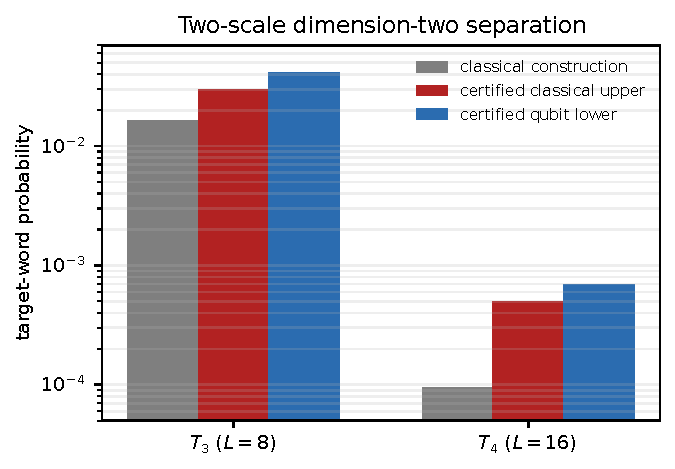
\includegraphics[width=\columnwidth]{figures/fig3_certified_separation.pdf}
  \caption{Certified equal-dimension separation at two recursive scales.
  Red bars are rigorous global classical upper thresholds; blue bars are
  rigorous explicit-qubit lower bounds.  Gray bars are feasible classical
  constructions and do not define the bounds.}
  \label{fig:separation}
\end{figure}

\section{Conditional robustness and finite samples}
\label{sec:robustness}

To make the statistical scale explicit, we freeze one trusted noise model.
At each round, with probability $1-\eta$ the ideal outcome map is applied;
with probability $\eta$, the device outputs a fair random bit and resets the
qubit to $I/2$.  This is a registered implementation model, not an
arbitrary-noise or device-independent statement.  Exact channel propagation
gives a crossing of the classical threshold at
\begin{equation}
  \eta_{\mathrm c}=0.085449325714\ldots .
\end{equation}
At $\eta=0.02$, the target probability is
$0.038402921993\ldots$ (Fig.~\ref{fig:noise}).

\begin{figure}[t]
  \centering
  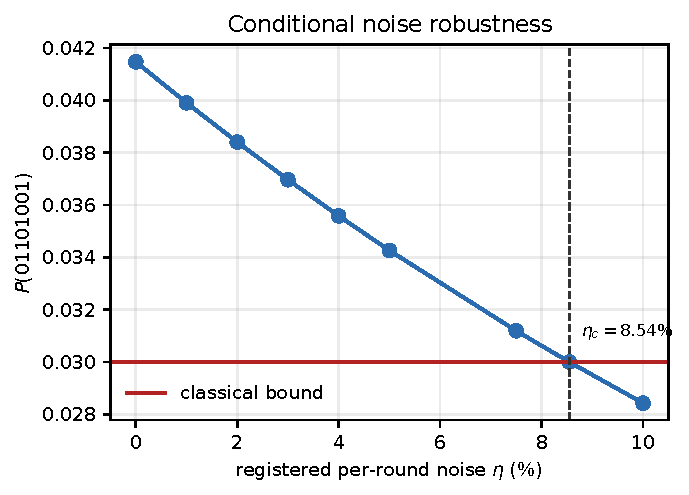
\includegraphics[width=\columnwidth]{figures/fig4_noise_robustness.pdf}
  \caption{Target-word probability under the frozen per-round reset-noise
  model.  Robustness outside this model is not claimed.}
  \label{fig:noise}
\end{figure}

For $m$ independent length-eight trials, let $X$ be the target-word count.
Testing the conservative null $p_0=0.03$ with an exact binomial upper-tail
test, a one-sided five-sigma type-I error and at least $90\%$ power require
$m=9957$ ideal trials, rejecting for $X\geq388$.  At $\eta=0.02$, the
corresponding design is $m=17979$ and $X\geq658$.  The achieved type-I errors
are $2.85\times10^{-7}$ and $2.82\times10^{-7}$, respectively.  These
figures do not include uncertainty in a physical dimension calibration or
violations of stationarity.

\section{Discussion}

\paragraph{What is certified.}
The result separates stationary two-state classical generators from explicit
stationary qubit instruments on two preselected members of one recursive
family.  Both classical bounds are global within the stated model and end in
exact rational verification.  The entire dyadic family has an exact
deterministic memory law.

\paragraph{What is not certified.}
A physical implementation would have to justify the dimension-two null and
exclude a hidden clock, time-dependent control, side channels, and
postselection.  The noise calculation is conditional.  The result does not
identify hidden quantum states, does not modify the Born rule, and does not
claim that the Thue--Morse substitution is a microscopic law of nature.

\paragraph{Relation to word complexity.}
Automatic complexity studies the smallest automata recognizing individual
finite strings \cite{ShallitWang2001}.  Our deterministic quantity belongs to
a different operational model: autonomous emission by one repeated
instrument with an external stop.  The distinction is essential for
recursive automatic sequences, whose compact index-reading descriptions
otherwise look like a contradiction to Theorem~\ref{thm:dc}.

\paragraph{Open problems.}
The most important next step is an asymptotic probabilistic separation for
the family $T_n$.  The two certified scales reported here establish
recurrence, not an asymptotic law.  On the classical side, sharper exact
bounds could be obtained with polynomial optimization or support
elimination.  On the quantum side, recursive instruments or matrix-product
constructions may expose a scalable ratio.  Experimentally, an
independently dimension-bounded platform and a preregistered stationarity
audit would turn Proposition~\ref{prop:separation} into a direct temporal
memory test.

\section{Conclusion}

Recursive complement structure can be simple for an index-reading automaton
yet memory intensive for an autonomous clock-free generator.  Finite
Thue--Morse words make this distinction exact:
$\DC(T_n)=3|T_n|/4$.  At the first two dyadic lengths beyond the prior
quantum survey, global classical certificates and explicit qubit instruments
give strict equal-dimension separations.  The construction supplies a
compact, reproducible temporal-memory witness with a clearly delimited
experimental route.

\paragraph{Data and code availability.}
All source code, exact certificate outputs, numerical witness data, plotted
data, and a one-command reproduction script are archived on Zenodo at
\href{https://doi.org/10.5281/zenodo.21695591}
{doi:10.5281/zenodo.21695591}.  The public source repository is available at
\href{https://github.com/youfuwang888-tech/recursive-temporal-memory-witnesses}
{github.com/youfuwang888-tech/recursive-temporal-memory-witnesses}.

\paragraph{Author contributions and AI-use disclosure.}
Y.W. originated the recursive-closure research direction, defined the
research objective, and is the sole human author responsible for the work.
OpenAI Codex was used under the author's direction for bibliographic
research, code and calculation implementation, theorem and manuscript
drafting, figure production, and formatting.  The author reviewed and
approved all final claims, code, and submitted materials and assumes full
responsibility for them.

\paragraph{Competing interests.}
The author declares no competing interests.

\appendix

\section{Full deterministic proof}
\label{app:proof}

Let $t=t_0t_1\ldots$ be the infinite Thue--Morse word.  It obeys
\begin{equation}
  t_{2i}=t_i,\qquad t_{2i+1}=1-t_i.
  \label{eq:tmidentities}
\end{equation}

\begin{lemma}[Odd displacements]
Two factors of $t$ separated by an odd displacement agree on at most three
consecutive symbols.
\end{lemma}
\begin{proof}
Every length-four factor beginning at an even position is the image under
$\mu$ of a length-two factor and belongs to
\[
\{0101,0110,1001,1010\}.
\]
Every length-four factor beginning at an odd position is fixed by a
length-three preimage factor and the one-symbol offset, and belongs to
\[
\{0010,0011,0100,1011,1100,1101\}.
\]
The sets are disjoint.  An odd displacement exchanges parity, so a
four-symbol match is impossible.
\end{proof}

\begin{lemma}[Even-displacement desubstitution]
If $q=2^s u$ with $u$ odd, a matching run at displacement $q$ has length at
most $2^s$ times the longest matching run at odd displacement after $s$
desubstitutions.
\end{lemma}
\begin{proof}
For displacement $2r$, Eq.~\eqref{eq:tmidentities} gives
\[
[t_{2i}=t_{2i+2r}]
=[t_{2i+1}=t_{2i+1+2r}]
=[t_i=t_{i+r}].
\]
Thus the equality-indicator word for $2r$ is obtained from that for $r$ by
duplicating every symbol.  A run of ones can grow by at most a factor two.
Iterating $s$ times proves the claim.  Restricting to the finite prefix
$T_n$ can only truncate a run.
\end{proof}

For $n-s\geq4$, the preceding lemmas bound a run by
$3\,2^s<2^{n-2}$.  Direct inspection of $T_3,T_2,T_1$ gives odd-shift
maxima $2,1,0$, respectively, and the same upper bound in all terminal
cases.  Hence $M(T_n)\leq2^{n-2}$.  Equation~\eqref{eq:fourblocks} attains
this value.

Any deterministic trajectory on $d$ states repeats a state among the first
$d+1$ visited states.  Its emitted word is therefore a tail followed by a
cycle with total tail-plus-cycle length at most $d$.  If it emits $N$
symbols, the last $N-d$ symbols match the block one cycle earlier, so
$N-d\leq M(T_n)$.  This yields $d\geq3N/4$.  The cycle construction following
Eq.~\eqref{eq:fourblocks} attains equality.  Complementation preserves every
equality relation, completing the proof of Theorem~\ref{thm:dc}.

\section{Exact-rational classical certificate}
\label{app:certificate}

For each source state, list the four joint outcome--destination
probabilities in the order
\[
(0,0),(0,1),(1,0),(1,1).
\]
The first three are independent variables $x_1,x_2,x_3\geq0$ with
$x_1+x_2+x_3\leq1$; the fourth is
$1-x_1-x_2-x_3$.  Repeating this for the second source state gives six
variables.

For a rational box $B=[\ell,u]$, feasibility tightening replaces each upper
endpoint by
\[
u_i\leftarrow\min\!\left(u_i,1-\sum_{j\neq i}\ell_j\right)
\]
within its simplex.  The independent transition entries are bounded by
$u_i$, and the dependent entry by $1-\sum_i\ell_i$.  Call the resulting
nonnegative entrywise upper matrices $\widehat T_0(B),\widehat T_1(B)$.
Starting from the pure initial state, positive matrix multiplication yields
an upper vector after every symbol.  The sum of its entries is therefore an
upper bound $U(B)$ on the target probability throughout $B$.

The algorithm begins with the two full simplices, removes infeasible boxes,
and bisects a widest rational interval at its midpoint.  Replacing one box
by its feasible children preserves coverage of the parameter domain.
Consequently, at every iteration,
\[
\sup_{\theta}P_{\mathrm C}(w;\theta)
\leq\max_{B\ \mathrm{queued}}U(B).
\]
All endpoints, propagation steps, comparisons used for the final bound, and
the final maximum are exact \texttt{Fraction} operations.  Floating-point
values are used only to prioritize the queue and cannot affect coverage or
the final inequality.  After $130000$ processed boxes the exact maximum is
Eq.~\eqref{eq:exactcertificate}.  Its distance below $3/100$ is exactly
\[
\frac{3}{100}
-\frac{16282708641}{549755813888}
=\frac{5249144391}{13743895347200}>0.
\]

For $T_4$, a faster first stage uses IEEE-754 operations with every
multiplication, addition, and simplex tightening rounded outward via
\texttt{nextafter}.  Best-first bisection leaves $176112$ boxes whose largest
outward upper bound is $0.000499999289033824\ldots$.  In a separate second
stage, every endpoint of every remaining box is converted to its exact
binary rational value and the full length-16 propagation is recomputed with
\texttt{Fraction} operations.  No box reaches $1/2000$; the largest exact
bound is $0.000499999289033821\ldots$.  Because every processed box is
replaced by its feasible children, the final queue retains the same coverage
invariant as above.  The exact numerator and denominator are included in the
machine-readable certificate rather than printed here.

\section{Classical feasible construction}

The best classical value found numerically lies on the support
\[
\begin{aligned}
T_0&=\begin{pmatrix}a&0\\1-a&a\end{pmatrix},&
T_1&=\begin{pmatrix}b&c\\0&0\end{pmatrix},\\
&&a+b+c&=1,
\end{aligned}
\]
with initial state $(0,1)$.  The target probability is
\begin{align}
P(a,b)={}&ab(a-1)^2(a^2+2ab-2a-b+1)\nonumber\\
&\times(2a^2+3ab-4a-2b+2).
\end{align}
The feasible stationary point has
\[
\begin{aligned}
a&=0.142664084620\ldots,\\
b&=0.326162782878\ldots,
\end{aligned}
\]
and gives $P=0.016434148019\ldots$.  This construction is a lower bound on the
classical optimum only and is not used in Proposition~\ref{prop:separation}.

\section{Quantum witness verification}
\label{app:quantum}

With one Kraus operator per outcome,
\[
\mathcal I_a(\rho)=K_a\rho K_a^\dagger.
\]
The archived machine-readable parameters retain the displayed decimal
definitions.  Positivity of $I-K_0^\top K_0$ is checked by interval
arithmetic.  The square-root completion makes trace preservation exact by
definition, while an independent 80-digit outward-interval computation
certifies $P_{\mathrm Q}>0.0414$.

For $T_4$, the same exactly normalized parameterization uses
\begin{align*}
\theta&=-0.35791546499923926,\\
\phi&=2.1733161717864493.
\end{align*}
\[
K_0=
\begin{pmatrix}
-0.293850518688&-0.219854695403\\
 0.862588464315&-0.314384115846
\end{pmatrix}.
\]
\[
K_1=R(\phi)\sqrt{I-K_0^\top K_0}.
\]
The residual eigenvalues are
$0.1119890568958\ldots$ and $0.9104304976137\ldots$.
An independent 80-digit outward-interval computation certifies
$P_{\mathrm Q}(T_4)>0.00069$.

\section{Exact-binomial design}

For $X\sim\mathrm{Binomial}(m,p)$, the rejection threshold is the smallest
integer $k$ satisfying
\[
\Pr_{p_0=0.03}[X\geq k]\leq\alpha.
\]
Power is $\Pr_{p_1}[X\geq k]$.  We search integer $m$ and $k$ directly,
without a normal approximation.  Table~\ref{tab:shots} records the frozen
designs.

\begin{center}
\refstepcounter{table}
\label{tab:shots}
\textbf{Table \thetable:} Exact-binomial designs with at least $90\%$ power.
\par\smallskip
\begin{tabular}{lrrrr}
\toprule
Condition & $\alpha$ & $m$ & $k$ & power\\
\midrule
ideal & $10^{-3}$ & 4877 & 185 & 0.90009\\
$\eta=0.02$ & $10^{-3}$ & 8788 & 315 & 0.90000\\
ideal & $2.87\,10^{-7}$ & 9957 & 388 & 0.90018\\
$\eta=0.02$ & $2.87\,10^{-7}$ & 17979 & 658 & 0.90018\\
\bottomrule
\end{tabular}
\end{center}

\begingroup
\small
\begin{thebibliography}{12}

\bibitem{VieiraBudroni2022}
L.~B. Vieira and C.~Budroni,
\href{https://doi.org/10.22331/q-2022-01-18-623}
{Temporal correlations in the simplest measurement sequences},
\textit{Quantum} \textbf{6}, 623 (2022).

\bibitem{Brierley2015}
S.~Brierley, A.~Kosowski, M.~Markiewicz, T.~Paterek, and
A.~Przysi\k{e}\.{z}na,
\href{https://doi.org/10.1103/PhysRevLett.115.120404}
{Nonclassicality of temporal correlations},
\textit{Phys. Rev. Lett.} \textbf{115}, 120404 (2015).

\bibitem{Budroni2019}
C.~Budroni, G.~Fagundes, and M.~Kleinmann,
\href{https://doi.org/10.1088/1367-2630/ab3cb4}
{Memory cost of temporal correlations},
\textit{New J. Phys.} \textbf{21}, 093018 (2019).

\bibitem{AlloucheShallit2003}
J.-P. Allouche and J.~Shallit,
\textit{Automatic Sequences: Theory, Applications, Generalizations}
(Cambridge University Press, 2003).

\bibitem{Deb2026}
P.~Deb, A.~Beige, and L.~A. Clark,
\href{https://arxiv.org/abs/2604.10315}
{Comparing quantum and classical finite state generators},
arXiv:2604.10315 (2026).

\bibitem{Vieira2024}
L.~B. Vieira, S.~Milz, G.~Vitagliano, and C.~Budroni,
\href{https://doi.org/10.22331/q-2024-01-10-1224}
{Witnessing environment dimension through temporal correlations},
\textit{Quantum} \textbf{8}, 1224 (2024).

\bibitem{Garner2017}
A.~J.~P. Garner, Q.~Liu, J.~Thompson, V.~Vedral, and M.~Gu,
\href{https://doi.org/10.1088/1367-2630/aa82df}
{Provably unbounded memory advantage in stochastic simulation using quantum
mechanics},
\textit{New J. Phys.} \textbf{19}, 103009 (2017).

\bibitem{Elliott2020}
T.~J. Elliott, C.~Yang, F.~C. Binder, A.~J.~P. Garner, J.~Thompson, and M.~Gu,
\href{https://doi.org/10.1103/PhysRevLett.125.260501}
{Extreme dimensionality reduction with quantum modeling},
\textit{Phys. Rev. Lett.} \textbf{125}, 260501 (2020).

\bibitem{ShallitWang2001}
J.~Shallit and M.-W. Wang,
\href{https://doi.org/10.25596/jalc-2001-537}
{Automatic complexity of strings},
\textit{J. Autom. Lang. Comb.} \textbf{6}, 537--554 (2001).

\bibitem{Ringbauer2017}
M.~Ringbauer and R.~Chaves,
\href{https://doi.org/10.22331/q-2017-11-25-35}
{Probing the non-classicality of temporal correlations},
\textit{Quantum} \textbf{1}, 35 (2017).

\bibitem{Sohbi2021}
A.~Sohbi, D.~Markham, J.~Kim, and M.~T. Quintino,
\href{https://doi.org/10.22331/q-2021-06-10-472}
{Certifying dimension of quantum systems by sequential projective
measurements},
\textit{Quantum} \textbf{5}, 472 (2021).

\bibitem{Taranto2023}
P.~Taranto, T.~J. Elliott, and S.~Milz,
\href{https://doi.org/10.22331/q-2023-04-27-991}
{Hidden quantum memory: Is memory there when somebody looks?},
\textit{Quantum} \textbf{7}, 991 (2023).

\end{thebibliography}
\endgroup

\end{document}
